% Generated figure assets; captions are suggestions for the manuscript author.
% Style/layout adaptation: Chen Liu, figures4papers, commit
% f0bb7559abe90f5e1828797126d4d133c1bd47d7, CC BY-NC 4.0.
\begin{figure}[t]
  \centering
  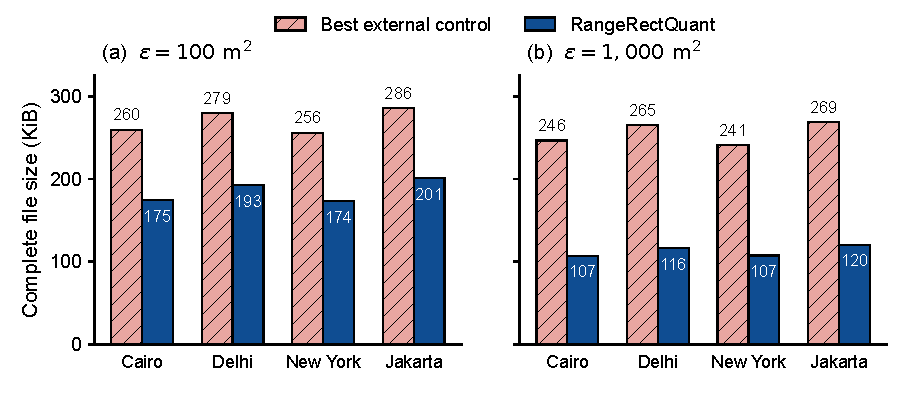
\includegraphics[width=\textwidth]{figures/heldout_rates.pdf}
  \caption{Complete file sizes on four geographically held-out windows.
  Each external bar is the smallest legal file in the fixed external control
  pool under the same rectangle-sum budget; the proposed method is frozen
  before acquisition. Sizes include all metadata, masks, and checksums;
  one KiB is 1,024 bytes. Bar labels are rounded to whole KiB.}
  \label{fig:heldout-rates}
\end{figure}

\begin{figure}[t]
  \centering
  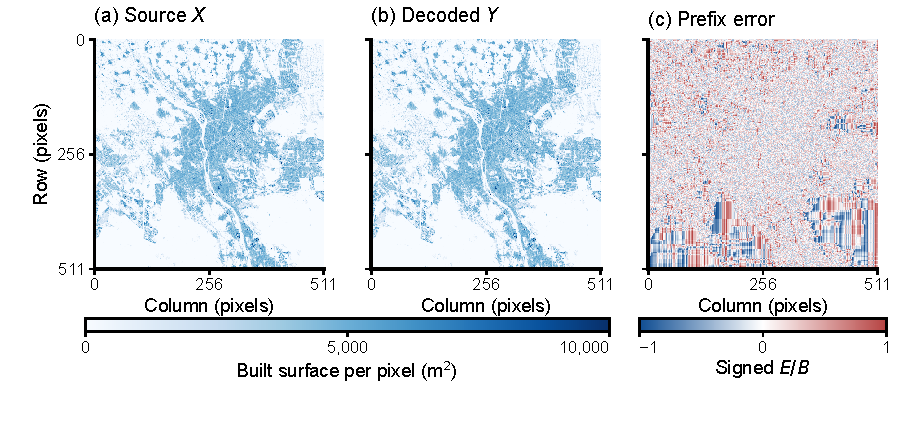
\includegraphics[width=\textwidth]{figures/field_example.pdf}
  \caption{A Cairo held-out window at $\epsilon=1{,}000$\,m$^2$ and coarse
  step $q=200$\,m$^2$. The original and saved decoded fields use the same
  built-surface scale and both remain integer-valued in $[0,10{,}000]$\,m$^2$.
  The right panel shows signed prefix error $E/B$, with $B=250$\,m$^2$;
  every displayed prefix lies in $[-B,B]$. All panels show the full
  $512\times512$ native-pixel window without a spatial crop.}
  \label{fig:field-example}
\end{figure}

\begin{figure}[t]
  \centering
  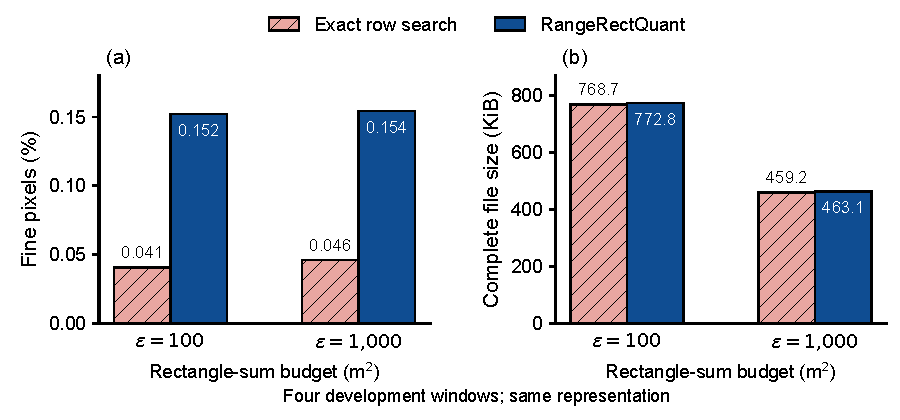
\includegraphics[width=\textwidth]{figures/precision_rate.pdf}
  \caption{Fine precision and complete rate on the four development windows
  only, using the same field carrier and default lossy mode for both methods.
  Fine samples are valid pixels whose decoded value is not divisible by $q$;
  percentages divide the aggregate fine count by $4\times512^2$ valid pixels.
  File sizes sum all four complete files. Row optimization reduces the fine
  count by 73.29\% and 70.21\%, but complete bytes by only 0.54\% and 0.85\%.
  Held-out carriers are not compared in this plot.}
  \label{fig:precision-rate}
\end{figure}
